\documentclass[a4paper, amsfonts, amssymb, amsmath, reprint, showkeys, nofootinbib, twoside]{revtex4-1}
\usepackage[english]{babel}
\usepackage[utf8]{inputenc}
\usepackage[colorinlistoftodos, color=green!40, prependcaption]{todonotes}
\usepackage{amsthm}
\usepackage{mathtools}
\usepackage{physics}
\usepackage{xcolor}
\usepackage{graphicx}
\usepackage[left=23mm,right=13mm,top=35mm,columnsep=15pt]{geometry} 
\usepackage{adjustbox}
\usepackage{placeins}
\usepackage[T1]{fontenc}
\usepackage{lipsum}
\usepackage{csquotes}
\usepackage[pdftex, pdftitle={Article}, pdfauthor={Author}]{hyperref} % For hyperlinks in the PDF
%\setlength{\marginparwidth}{2.5cm}
\bibliographystyle{apsrev4-1}

\begin{document}
\title{Self-assembly of finite size capsules using SAT-assembly}

\author{Diogo E. P. Pinto$^1$, Petr $\check{\text{S}}$ulc$^2$, Francesco Sciortino$^1$ and John Russo$^1$}
    \email[Correspondence email address: ]{john.russo@uniroma1.it}% Your name
    \affiliation{$^1$Dipartimento di Fisica, Sapienza Universit\`{a} di Roma, P.le Aldo Moro 5, 00185 Rome, Italy}
    \affiliation{$^2$School of Molecular Sciences and Center for Molecular Design and Biomimetics, The Biodesign Institute, Arizona State University, 1001 South McAllister Avenue, Tempe, Arizona 85281, USA}

\date{\today} % Leave empty to omit a date

\begin{abstract}
Inspired by Nature, the self-assembly of complex structures has been a longstanding challenge of material science. Self-assembly encompasses a large array of phenomena through which materials can be formed using microscopic building blocks which follow simple assembly rules. One example of these building blocks are patchy particles, which are commonly characterized by a hard core coated by one or more patches that interact attractively. By coloring each patch and treating the system as a color-color interaction problem, we are able to reformulate it as a SAT problem and use highly optimized computer science tools to solve the assembly process by inverse design. In this work, we use SAT on a patchy particle system with valence five to assemble finite size polyhedrons. SAT solvers can quickly find a suitable design for the assembly problem and calculate a color arrangement that leads to a targeted finite size polyhedron shell. We find that one can significantly improve the self-assembly yield of the most trivial color arrangements. We also show that these designs are robust to patch widths and geometries on the particle. Furthermore, we also highlight how this tool can be used to exclude competing structures, thus more efficiently target the desired finite size polyhedron shell.
\end{abstract}

\maketitle

\section{Introduction}

The assembly of complex structures through the use of minimalist building blocks has been a longstanding challenge of material science \cite{Bishop2022}. Self-assembly encompasses a large array of phenomena through which materials are formed through the use of simple assembly rules of microscopic building blocks \cite{Whitelam2015}. Nature has many striking examples where this type of assembly is successful \cite{Whitesides2002, Parnell2015, Teyssier2015}. In the case of synthetic materials, although quite a complex process, some realizations have been already successfully assembled, from three-dimensional crystals to polyhedral shells \cite{Dziomkina2005, Glotzer2007, Kim2011, LaCour2022,  McGorty2010, Mu2022, Nykypanchuk2008, Sacanna2011, Wang2012, Wang2015, Joshi2016}. One of the main difficulty resides in how to optimize the geometrical properties or interactions between the building blocks of a given material without leading to a kinetically arrested configuration \cite{Frenkel2011, Lash2015, Blaaderen2006, Meulen2015}.

Recently a novel technique has been proposed which strives to answer this question. By describing the assembly as a constraint satisfiability problem (SAT), one is able to apply general tools to target the desired structures and exclude competing ones \cite{Romano2020a}. Its most successful application in this field is in the assembly of patchy particles, where the building blocks are considered hard spheres with attractive patches on its surface \cite{Bianchi2006, Romano2010, Rovigatti2018, Russo2021, Sciortino2009}. These represent a coarse-grained approach to describe multiple systems, e.g. colloids, proteins, polymers, etc \cite{Sacanna2011, Wang2012}. If to each patch is associated a color, one can create an array of constraints that satisfy the topology of a given target structure \cite{Russo2021a}. This is where SAT solving tools come in, since they have been created to efficiently solve these problems and come up with a solution that satisfies the constraints imposed \cite{Een2005}.

Previous work has focused on the assembly of crystals and how to overcome its competing structures \cite{Romano2020a}. Here, we focus on the finite size structures and use SAT to target specific polyhedron shells. When focusing on finite size shells, new problems arise since one requires the shell to fully close. For example, drug delivery systems have been a widely research topic where a given drug is encapsulated within a closed shell and then driven to a specific diseased area in order to locally release the drug and affect the least amount of non diseased tissue \cite{Huang2007, Uchida2007}. For this, the shell needs to be able to close around a specific reagent and then open when external conditions are met. Recently, there have been suitable experimental realisations of this, for example, using DNA-origami, where selective interactions can be introduced to mimic the same rules as in patchy particles \cite{Mosayebi2017, Lee2022, Jun2021, Rothemund2006}. By combining this with SAT we open the doors for a robust assembly process, since we can use it to discard competing polyhedron shells and make sure that a given combination of patchy particle species which differ on the coloring of their patches lead to the targeted shell.

In this work we focus on patchy particles with a valence of 5 (number of patches on the surface of the sphere) and explore how one can tackle the problem of finite size assembly using SAT. We start by discussing the patchy particle model used and how SAT is applied to it. Then we detail the finite size shells found using an almost trivial solution given by SAT and how to control the geometrical and interaction parameters to bias the different configurations. We then discuss the thermodynamics of the systems and highlight the phase separation between the liquid and gas phase, similar to other patchy particle systems \cite{Sciortino2009}. Finally we conclude by showing how to push SAT to target, in an efficient way, a given polyhedron shell. We conclude with a discussion and an outlook.

\section{Model}

We consider a system composed of $N$ patchy particles in a cubic box of length $L$. The particles are characterized by a hard core of radius $\sigma$ with five patches on its surface. The patches interact through the Kern-Frenkel portential \cite{Kern2003}:

\begin{equation}
Vpp(\boldsymbol{r}_{ij}, \boldsymbol{\hat{r}}_{\alpha, i}, \boldsymbol{\hat{r}}_{\beta, j})=V_{SW}(r_{ij})f(\boldsymbol{r}_{ij}, \boldsymbol{\hat{r}}_{\alpha, i}, \boldsymbol{\hat{r}}_{\beta, j})
\end{equation}

where $i$ corresponds to a given particle and $\boldsymbol{r}_{i}$ its center of mass. Thus, $\boldsymbol{r}_{ij}$ is the distance between particles $i$ and $j$. $\boldsymbol{r}_{\alpha, i}$ denotes the position of patch $\alpha$ of particle $i$. $V_{SW}$ is an isotropic square-well of range $\sigma + \delta_{\alpha,\beta}$ and depth $\varepsilon_{\alpha,\beta}$, the hat symbol indicate unit vectors and $f$ is the orientation-dependent modulation term that takes the form:

\begin{equation}
\label{KF}
f(\boldsymbol{r}_{ij}, \boldsymbol{\hat{r}}_{\alpha, i}, \boldsymbol{\hat{r}}_{\beta, j})=
    \begin{cases}
        1 & \text{if $\begin{aligned}
            \text{$\boldsymbol{\hat{r}}_{ij} \cdot \boldsymbol{\hat{r}}_{\alpha, i} > \cos     \theta^{max}_{\alpha \beta}$} \\
            \text{$\boldsymbol{\hat{r}}_{ji} \cdot \boldsymbol{\hat{r}}_{\beta, j} > \cos     \theta^{max}_{\alpha \beta}$}
        \end{aligned}$ } \\
        0 & \text{otherwise}
    \end{cases}
\end{equation}

With this formulation patches are represented by a cone starting from the center of mass of the particle and reaching $\sigma + \delta_{\alpha,\beta}$, while the width is controlled by $\theta^{max}_{\alpha \beta}$. This potential has been extensively used to study systems of patchy particles \cite{Rovigatti2018}. For simplicity, we consider the parameter range where it is only possible to form one bond per patch. In the following, $\sigma$ provides the unit of length and $\varepsilon_{\alpha, \beta}$ the unit of energy. Temperature ($T$) is also expressed in units of $\varepsilon_{\alpha, \beta}$, with $k_B=1$.

For the following results we considered Monte Carlo (MC) simulations with two possible moves, rototranslations and aggregation-volume-bias. The first attempts a simple rotation and translation of a random particle along a random (radial or angular) direction. The second, attempts to move a random particle into the vicinity of another such that a bond is formed between the two. To not break ergodicity, the inverse move can also be performed where a random bond between two particles is broken. We performed simulations in the $NVT$ assemble to explore the assembly of our desired shells and also performed simulations in the $NPT$ and $Gibbs$ assembles to explore the different thermodynamic phases of the model. All results shown bellow were averages over simulations with or more than $10^8$ MC time-steps. For all, we considered $N=480$ and $\delta_{\alpha, \beta}=0.2$. The simulations start with particles randomly generated in the box with random orientations. Unless stated otherwise, all results are averages over $10$ samples.

We follow the same SAT formulation as the one in Ref.~\cite{Russo2021}. We consider that each patch can have a given color between $1\leq x_c\leq N_c$, where $N_c$ is the total number of colors. These colors can be distributed onto the patches in specific arrangements, each unique sequence can be considered a particle specie, thus $1\leq x_p\leq N_p$, where $N_p$ is the total number of species. SAT is then used to find if a given combination of $N_p$ and $N_c$ can satisfy a given polyhedral shell, e.g. if it satisfies all the topological constraints, and a solution is calculated which can be used to prepare the composition of the system. In the \emph{Supplemental Material} we go into more detail on the different constraints (clauses) used in SAT.

In Fig~\ref{SAT} we have a schematic showing the patchy particles used and the different configurations assembled. There are three possible polyhedron shells that can form and fully close, depending on the parameters and SAT solution used: the regular icosahedron, the snub cube and the snub dodecahedron. We consider the assembly of patchy particles of valence five. The positions of the patches, in the orthonormal base associated with the patchy particle, are given as:

\begin{equation}
    \label{patch}
    \begin{aligned}
    \textbf{p}_1=(-0.698, 0.186, -0.691) \\
    \textbf{p}_2=(-0.502, -0.756, -0.419) \\
    \textbf{p}_3=(-0.123, -0.857, 0.5) \\ 
    \textbf{p}_4=(-0.410, -0.007, 0.912) \\
    \textbf{p}_5=(-0.751, -0.627, 0.204) .
    \end{aligned}
\end{equation}

\noindent for the case of the icosahedron. To form the other structures one can increase the in plane angle between $\textbf{p}_4$ and $\textbf{p}_5$ while maintaining the remaining ones. In the next section we explore how this geometrical change plays a role in the assembly process. We look at different in plane angles between these two patches ranging from the minimum of $60$ degrees, for the icosahedron, to the maximum of $108$ degrees, for the snub dodecahedron.

Using SAT we can find a minimal design that satisfies all three structures. For example, it is possible to consider the case that is shown in Fig.~\ref{SAT}, where we only use one specie (blue) of particles and two colors (green and red) for patches. For this design, green patches only interact with green and red with red. If the particles follow this coloring and interactions then the three structures can form. The solution that leads to this design is not necessarily the only one that satisfies all structures but SAT only provides one solution at a time for the constraints provided. Nonetheless it is flexible enough, such that, we can provide this solution found as a new constraint and thus avoid it altogether leading to new solutions. This process can be iterated until all solutions are exhausted. We will first focus on this design with one specie and two colors to explore how the interaction and geometry of the patches plays a role in the assembly. We will also use it to explore the phase behavior of this patchy particle system. Then, we will use SAT to target specific shells in order to highlight the true use of SAT as a robust predicting tool.

\begin{figure}[t]
	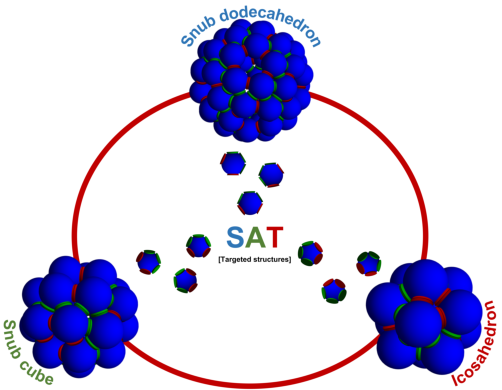
\includegraphics{fig1.pdf}
	\caption{\label{SAT} Schematic representation of the structures explored. A particle with valence 5 is used to assemble the different polyhedron shells. A solution calculated with SAT is used for the patchy particle design which satisfies all three structures. It contains only one particle specie (blue) and two patch colors (green and red). The green patches only interact with green while the red only interact with red.}
\end{figure}

\section{Results}

As a first approach to the assembly problem posed in Fig.~\ref{SAT}, we consider the most trivial design possible: one particle type and one patch color. Due to its simplicity we do not require the help of SAT to design the patchy particles. Using the simulation scheme detailed in the previous section we explore different values for the patch width, $\cos\theta_{max}$ (in Eq.~\ref{KF}, where we drop $\alpha$ and $\beta$ for simplicity) as well as different geometries of the patches by changing the in plane angle created by $\textbf{p}_4$ and $\textbf{p}_5$ in Eq.~\ref{patch}. The former allows for more flexibility of the bonds due to larger patch widths. The latter improves our ability to target the different structures proposed in Fig.~\ref{SAT} by more easily satisfying their topology. For example, if the in plane angle between these vectors is close to $90$ degrees it is easier to form the squares in the snub cube.

Figure \ref{N1c1} shows the results measured for the trivial solution. It shows the most probable structure found out of the ones shown in Fig.~\ref{SAT}. If none of them is formed then we classify the clusters into two groups. The black crosses correspond to incomplete clusters, the ones where particles form bonds but they do not close, thus forming an open shell. The gray stars correspond to irregular polymorphs, thus clusters that form and are able to completely close but are not any of the ones in Fig.~\ref{SAT}. They are irregular in the sense that they do not correspond to any specific polyhedron. We find that only the icosahedron is able to form for the range of parameters explored. Furthermore, increasing patch width (lowering $\cos\theta_{max}$), thus increasing bond flexibility hinders the assembly of these structures. From these results we can conclude that it is not sufficient for a particle and patch design to satisfy the targeted structure for it to assemble.

\begin{figure}[t]
	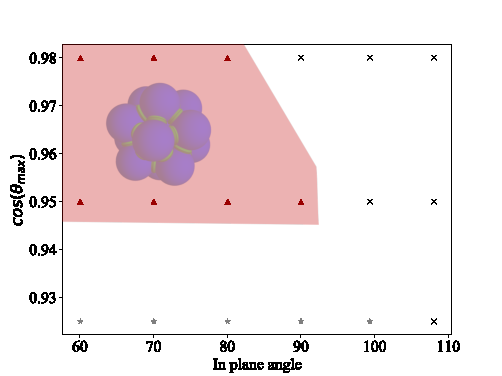
\includegraphics{fig2.pdf}
	\caption{\label{N1c1} Most probable structure formed for different in plane angles of $\textbf{p}_4$ and $\textbf{p}_5$ in Eq.~\ref{patch} and for different patch width, $\cos\theta_{max}$, in Eq.~\ref{KF}. The triangles inside the red region represent parameters where the most probable polyhedron shell from the ones in Fig.~\ref{SAT} is the icosahedron. Black crosses represent systems where only open/incomplete clusters are formed. The gray stars represent systems where clusters are able to close but none correspond to the ones in Fig.~\ref{SAT}. We find that for the most trivial solution only the icosahedron is able to form.}
\end{figure}

We now consider a non trivial design but with minimal colors and species. We use SAT to calculate a solution that satisfies all three structures but with only one particle specie and two patch colors, as shown in Fig.~\ref{SAT}. This solution dictates the patch design (which color has a given patch) and the interactions, which in this case are all self-similar (red with red and green with green). In Fig.~\ref{N1c2} are the results accompanied by some typical configurations. Using this design we can identify the three different structures from Fig.~\ref{SAT} within the parameters explored. Examples are shown with the snapshots of the system on the right. Thus, one can significantly improve on the trivial solution by using SAT as a design tool to assemble finite size shells, even with minimal colors and species. These results also suggest that as patch width increases, structures with fewer particles are favored. Since structures with fewer particles are easier to form and close, the patch width compensates for the changes in geometry of the patches.

\begin{figure}[t]
	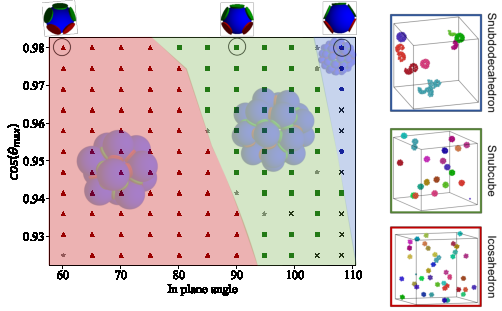
\includegraphics{fig3.pdf}
	\caption{\label{N1c2} Most probable structure formed for different in plane angles of $\textbf{p}_4$ and $\textbf{p}_5$ in Eq.~\ref{patch} and for different patch width, $\cos\theta_{max}$, in Eq.~\ref{KF}. The triangles inside the red region represent parameters where the most probable structure from the ones in Fig.~\ref{SAT} is the icosahedron. The squares inside the green region represent parameters where the most probable structure from the ones in Fig.~\ref{SAT} is the snubcube. The pentagons inside the blue region represent parameters where the most probable structure from the ones in Fig.~\ref{SAT} is the snub dodecahedron. Black crosses represent systems where only open/incomplete clusters are formed. The gray stars represent systems where clusters are able to close but none correspond to the ones in Fig.~\ref{SAT}. On top of the plot are schematics of three different particles with the corresponding colors. The left one has an in plane angle of $60$ degrees, the middle of $90$ degrees and the right one of $108$ degrees. On the right are typical configurations from the parameters that are encircled in the plot. They were imaged with OVITO and the colors represent different clusters. The design used was of one specie and two colors, where all interactions are self-similar (red with red and green with green).}
\end{figure}

Figure \ref{Yield} shows the different yields of the polyhedron shells using the most optimized in plane angle for each ($60$ degrees for the icosahedron, $90$ degrees for the snubcube and $108$ degrees for the snub dodecahedron). We define the yield as the probability of finding a cluster corresponding to a specific structure. We count single particles as a cluster of size one and any bonded particles as clusters of size two or above, depending on the number of particles bonded. We find that for this solution the snub cube has the highest yield for all the densities explored except the last one.  We hypothesize that in very high densities, structures with less particles are easier to assemble given that they occupy less space. On the other hand, large structures like the snub dodecahedron, which is composed of $60$ particles, is better assembled in very dilute systems where larger shells have more space to grow without influencing each other. The fact that the yield of the snub cube is higher than the icosahedron, even though its shell is larger, might be due to the specific design used. In the case of the snub cube, the patchy particle geometry is already asymmetrical and the solution used helps enforce it in the assembly, thus the clusters that are not snub cubes are incomplete shells. On the other hand, the icosahedron patchy particle has some rotational symmetries. For example, if every patch has the same color, one can rotate each particle as a rigid body four times while still satisfying the same topology. In the design with two colors, this symmetry is lost. For the particles to satisfy the topology of the assembly, each needs to have specific orientation, thus losing the rigid body rotational symmetry given by the patch positions. This leads to many clusters which are formed with twelve particles (the number of particles in the icosahedron) but with one or two bonds missing for it to fully close.

\begin{figure}[t]
	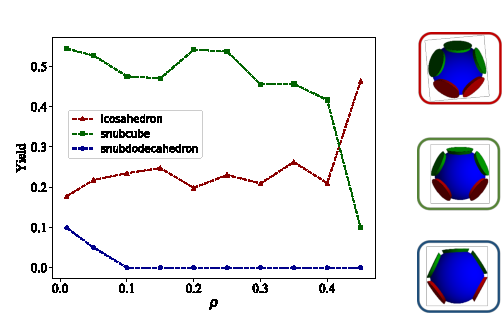
\includegraphics{fig4.pdf}
	\caption{\label{Yield} Average yield of the three different structures in Fig.~\ref{SAT} as a function of the density of patchy particles in the box. These results were calculated with $\cos\theta_{max}=0.98$ and the in plane angle was chosen to be the best for each structure. Thus, the icosahedron curve was calculated with an in plane angle of $60$ degrees, the snub cube with an in plane angle of $90$ degrees, while the snub dodecahedron with $108$ degrees. For these results the one specie and two colors design was used, as shown in Fig.~\ref{SAT}. On the right are schematic representations of the geometries of the corresponding patchy particles. }
\end{figure}

\begin{figure*}[t]
	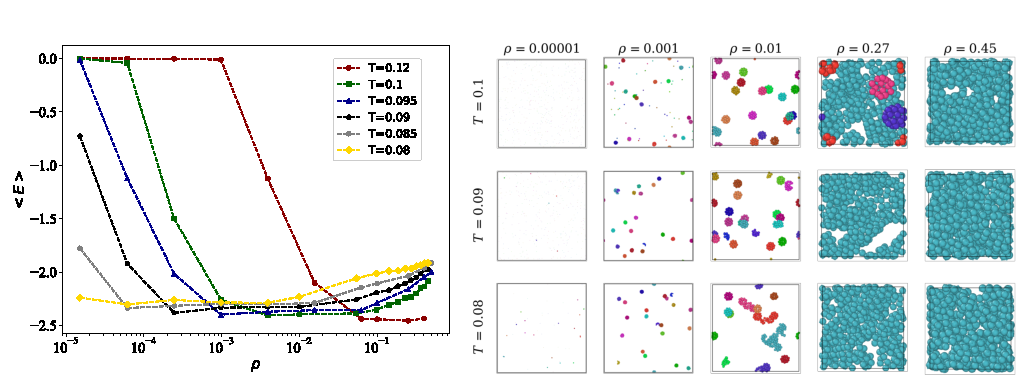
\includegraphics{fig5.pdf}
	\caption{\label{Energy} (Left) Average potential energy per particle as a function of density for different isotherms. For clarity, the x-axis is in log-scale. We observe a non monotonic behaviour of the average energy characteristic of self-assembly systems. (Right) Frontal snapshots of the system for different densities and temperatures. Images were obtained with OVITO, where the colors represent particles that belong to the same cluster. For low densities, some colors repeat themselves even though particles are not bounded due to the large number of unbounded particles which count as clusters of size one. All results were simulated with the one specie and two color design, with an in plane angle of $90$ degrees and a $\cos\theta_{max}=0.98$.}
\end{figure*}

Given the simplicity of this solution we also present a simple study of the phase behavior of this patchy particles in Fig.~\ref{Energy}. As a first approach we restrict ourselves to the parameters $\cos\theta_{max}=0.98$ and an in plane angle of $90$ degrees. This combination favors the snub cube shell as presented above. We observe a non-monotonic behavior of the average energy as a function of density, characteristic of self-assembly systems \cite{Sciortino2009}. For low densities there is an entropic gas phase where most particles are unbounded. As density increases or temperature decreases, more clusters will be formed. For intermediate densities we observe the minimum of the energy which corresponds to a gas of snub cubes. Here, the density is large enough and the temperature low enough for particles to bound and remain bounded until a snub cube is formed. These shells are the equilibrium structures for the patchy particles used which leads to the gas of clusters. For large densities, the liquid phase is approached and less clusters are formed leading to an increase of the average energy. Eventually the liquid phase percolates the system.

Lastly, we focus on a more complex design with two species and five colors. In this case we force SAT to calculate a solution that only satisfies one of the structures of Fig.~\ref{SAT}. Figure \ref{Sol} shows the results with the corresponding design in the images of the shells. Using SAT it is possible to generate solutions which exclude specific structures. Thus, one can, for example, calculate a solution that satisfies the topological constraints of the icosahedron but does not of the snub cube or snub dodecahedron. With this method, we prove that one can not only increase the range of parameters where a certain shell is formed but we also increase its yield, since it is more rare to find competing structures. Both for the icosahedron and snub cube designs we observe the increase of the parameter ranges over more in plane angles as well as $\cos\theta_{max}$, meaning that they are much more resilient to changes in the geometry of the patches and width of the interactions. On the other hand, the snub dodecahedron design does not change substantially the diagram compared to Fig~\ref{N1c2}. In this case, although the two species and five colors solution only satisfies the snub dodecahedron, one of the species, by itself, is able to form the other shells. We hypothesize that this will always be the case for any design, since the topology of the snub dodecahedron is almost the same as the snub cube, in term of which bonds are formed between particles and their orientations. Only one particle is the exception which is necessary to close the snub dodecahedron and not the snub cube. Thus, in any design with more than one species that satisfies the snub dodecahedron, there will be a subset of those species that will always satisfy the snub cube as well. We have explored all solutions in the two species case, varying the number of colors from two to ten, and none was found which satisfies the snub dodecahedron but its subsets do not satisfy any other structure (icosahedron or snub cube). One could try to exhaust (by brute force) all possible species and color combinations but as species and colors increase so do the number of solutions (and its subsets) making this a very demanding task.

\begin{figure*}[t]
	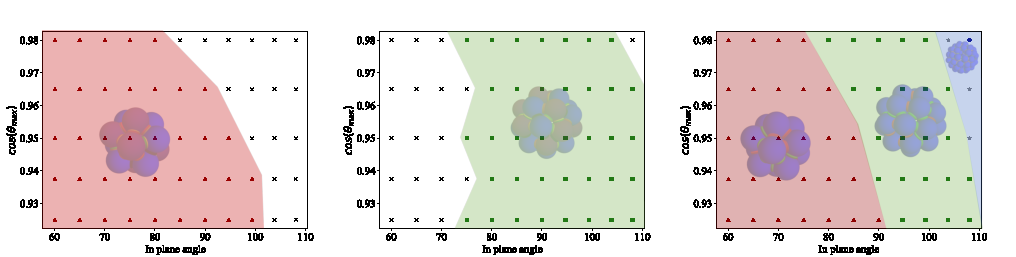
\includegraphics{fig6.pdf}
	\caption{\label{Sol} Most probable structure formed for different in plane angles of $\textbf{p}_4$ and $\textbf{p}_5$ in Eq.~\ref{patch} and for different patch width, $\cos\theta_{max}$, in Eq.~\ref{KF}. Here, each shell if formed using a two species and five colors design which only satisfies each of the structures shown. On the left the design only satisfies the icosahedron, in the middle the snub cube and on the right the snub dodecahedron. In the last picture all the shells are formed even though the design only satisfies the snub dodecahedron. This is because one single particle specie is enough to form the other structures.}
\end{figure*}

\section{Conclusion}

In this work we have shown how to translate the self-assembly of finite size structures using patchy particles into a SAT problem. Using patchy particles of valence five we explored different structures through Monte Carlo simulations and how to optimize the parameters to enhance self-assembly. We have proved that doing the most trivial design of patchy particles (one specie and one color) is worse than using SAT. While the most trivial design only yields one of the possible three shells, by slightly increasing the complexity of the design (adding one color) and allowing SAT to color the patches we find an overall improvement. The SAT design not only increases the probability of forming the finite size structures but allows us to also explore different structures by tuning the geometry or width of the patches. Thus, we show that with this patchy particles one can form the icosahedron, snub cube or snub dodecahedron. We also show how these structures are affected by density, showing that larger structures are harder to assemble in higher densities and smaller ones, like the icosahedron, are favored due to their small size leading to an increase in yield.

We also explored the phase diagram of these patchy particles designed with SAT. We find a non-monotonous behavior of the average potential energy as a function of density, as is typical of self-assembly systems \cite{Sciortino2009}. These results suggest a first entropic gas phase at very low densities, followed by a gas phase of clusters near the energy minima, ending at the liquid phase at high densities. We also show evidence of a liquid-gas coexistence region. Future studies should focus on a systematic study of the phase diagram to understand how different species and colors change the different phases, especially when taking into account different SAT designs.

Lastly, we used SAT to target only one of the structures previously assembled. For this, we increased the complexity of the design by increasing to two particle species and five patch colors. We use SAT to calculate particle designs that only satisfy one of the structures while excluding the others. We observe that for the icosahedron and snub cube, the designs obtained only satisfy these structures. Due to that the yield increases and we also find a wider parameter range where it is possible to successfully assemble these structures. On the other hand, while it is possible to find a design that only satisfies the snub dodecahedron, all of its subsets do not. Thus, one of the particle species, by itself, can always assemble one (or both) of the other structures. This results in a diagram of assembled structures which is similar to the previous one specie and two colors one. We argue that this happens due to the particular topology of the snub dodecahedron. It is always possible to take a subset of particles of this structure to form the other ones. Although we do not know of a mathematical prove to this, our results suggest it. We find no solutions in the two species case (and colors varying from two to ten) that satisfies the snub dodecahedron, where any subset of it does not satisfy the others. One could try to brute force higher particle species but this also increases the number of solutions that need to be tested making it a very demanding task.

Although we have only shown results for patchy particles of valence five, we have been able to successfully assemble other structures with different valences. It would be interesting to explore if similar permutations between structures is possible in other valences. With fewer patches the structures will need more parameter optimization to assemble since the number of bonds per particle is fewer and thus the structures can be less stable while forming. This might increase the probability of being stuck in kinetic traps.

One of the possible pathways of realizing these designs experimentally is through 3D DNA nanomaterials and in particular wireframe DNA origami. Previous studies have successfully shown the versatility of these materials in assembling a wide array of structures \cite{Mosayebi2017, Lee2022, Jun2021, Rothemund2006}. Furthermore, through the use of complementary strands one can functionalize the wireframe to act as a patchy particle with selective spatial bonding and tune the interactions accordingly \cite{Biancaniello2005, Wang2015}. We also argue that our results support such approach not only due to the high yields observed in simulations, but also due to the robustness of the structures formed to flexibility of the bonds, which is characteristic of DNA bonds \cite{Meulen2015, Meulen2015, Geerts2010}.

A demanding question would be to find a way to predict which design is better when using SAT. One of the gaps in this formulation is that there is no apriori knowledge which structures can form for a given SAT design. This comes only from intuition or after testing a given design in simulations. This requires a feedback loop between SAT and simulations that can be quite demanding, depending on the number of possible structures formed with the same design. Thus, finding apriori which designs generate configurations with the lowest energy would be of interest to not only self-assembly but also many other fields that deal with complex and disordered systems \cite{Franz2017}.

SAT has already been applied as an inverse assembly tool to form crystals and now in finite size structures. This proves the resilience of SAT for inverse self-assembly problems. Future studies will also focus on exploring other possible materials and structures that so far have been quite challenging to assemble. For example, SAT can become a useful tool in the assembly of quasi-crystals where the lack of translation symmetry (like in the crystal) makes the assembly process a daunting task \cite{Shechtman1984}. Recent studies have managed to simulate patchy particle systems which are able form quasi-crystals \cite{Noya2021}. Unfortunately, there is still a large degree of complexity in choosing the optimal design for targeting specific quasi-crystals, making it difficult to systematically change between structures without doing demanding simulation work first that is highly based on trial and error. SAT can help in this front, by creating a consistent algorithm that can find the appropriate design to target the specific structure without any previous trial and error task.

\section{Acknowledgements}

The authors acknowledge all the financial support from the European Research Council Grant DLV-759187.

\bibliography{refs}

\end{document}
